\documentclass[12pt]{article}
\usepackage[utf8]{inputenc}

\newenvironment{sol}[1][Solution]{\begin{trivlist}\item[\hskip\labelsep {\bfseries #1:}]}{\end{trivlist}}
\usepackage[margin=1in]{geometry} 
\usepackage{amsmath,amsthm,amssymb}
\usepackage{minted}
\usemintedstyle{vs}
\usepackage{graphicx}
\graphicspath{{./images}}
\usepackage{ amssymb }
\usepackage{times, url}
\usepackage{hyperref}

\title{CS7381 Project 5: Verilog Code Development – MIPS ALU Design }

\author{
Name: Bingying Liang \\
ID: 48999397\\  
Distance}
\date{March 31 2023}
\begin{document}
\maketitle
\noindent In the previous project (Project 4), you were introduced to the Verilog code development using the Cadence Xcelium tool. Next, we will use Verilog to modify the basic MIPS ALU of Project 4 and simulate this modification. \textbf{NOTE: for additional Verilog resources, please see my web \href{https://s2.smu.edu/~manikas/CAD_Tools/Verilog/Xcelium.htmlLinks to an external site.}{link}}

\begin{enumerate}
    \item Create a copy of the \href{https://smu.instructure.com/courses/106177/files/7251184?wrap=1}{S23\_MIPS\_ALU\_basic.v} file from Project 4. Similar to the MARS assignment, name your file using the first initial of your first name and the first 4 letters of your last name. For example, my ALU file name would be \textbf{tmani.v}.
    \begin{center}
        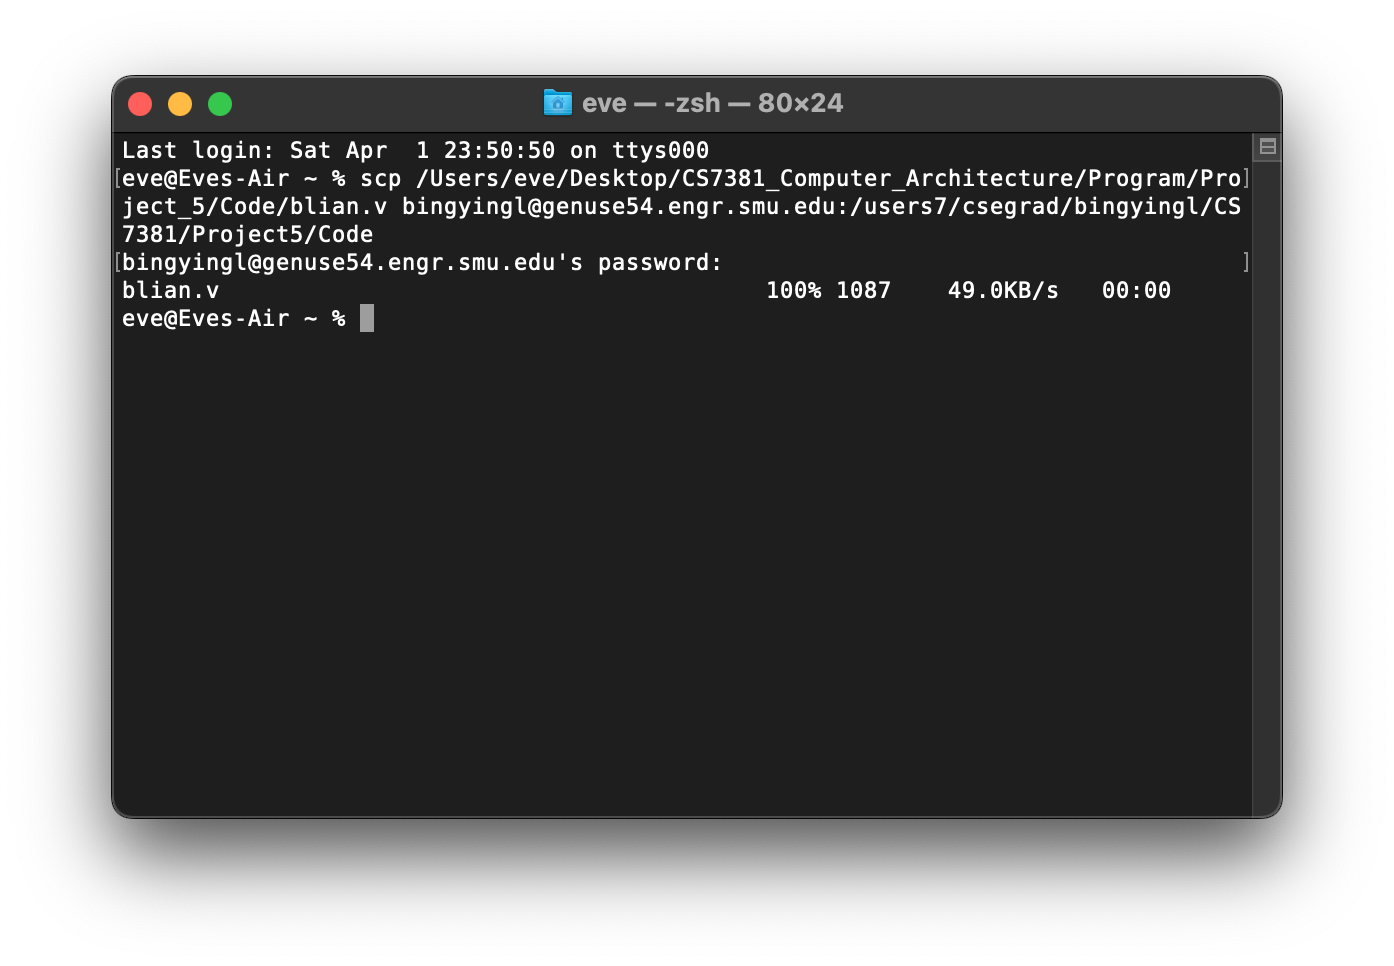
\includegraphics[width=0.9\textwidth]{p1.png}
    \end{center}
    
    \item \textbf{Add} the following functions to the ALU:
    \begin{enumerate}
        \item Function code 0 to implement bitwise AND: $A\ and \ B$
        \item Function code 2 to implement ADD $(A + B)$
        \item Function code 6 to implement SUB $(A - B)$
        \item Function code 12 to implement bitwise NOR $(A \ nor \ B)$
        \item Function code 14 to implement bitwise XOR $(A \oplus B)$
    \end{enumerate}
        \begin{center}
        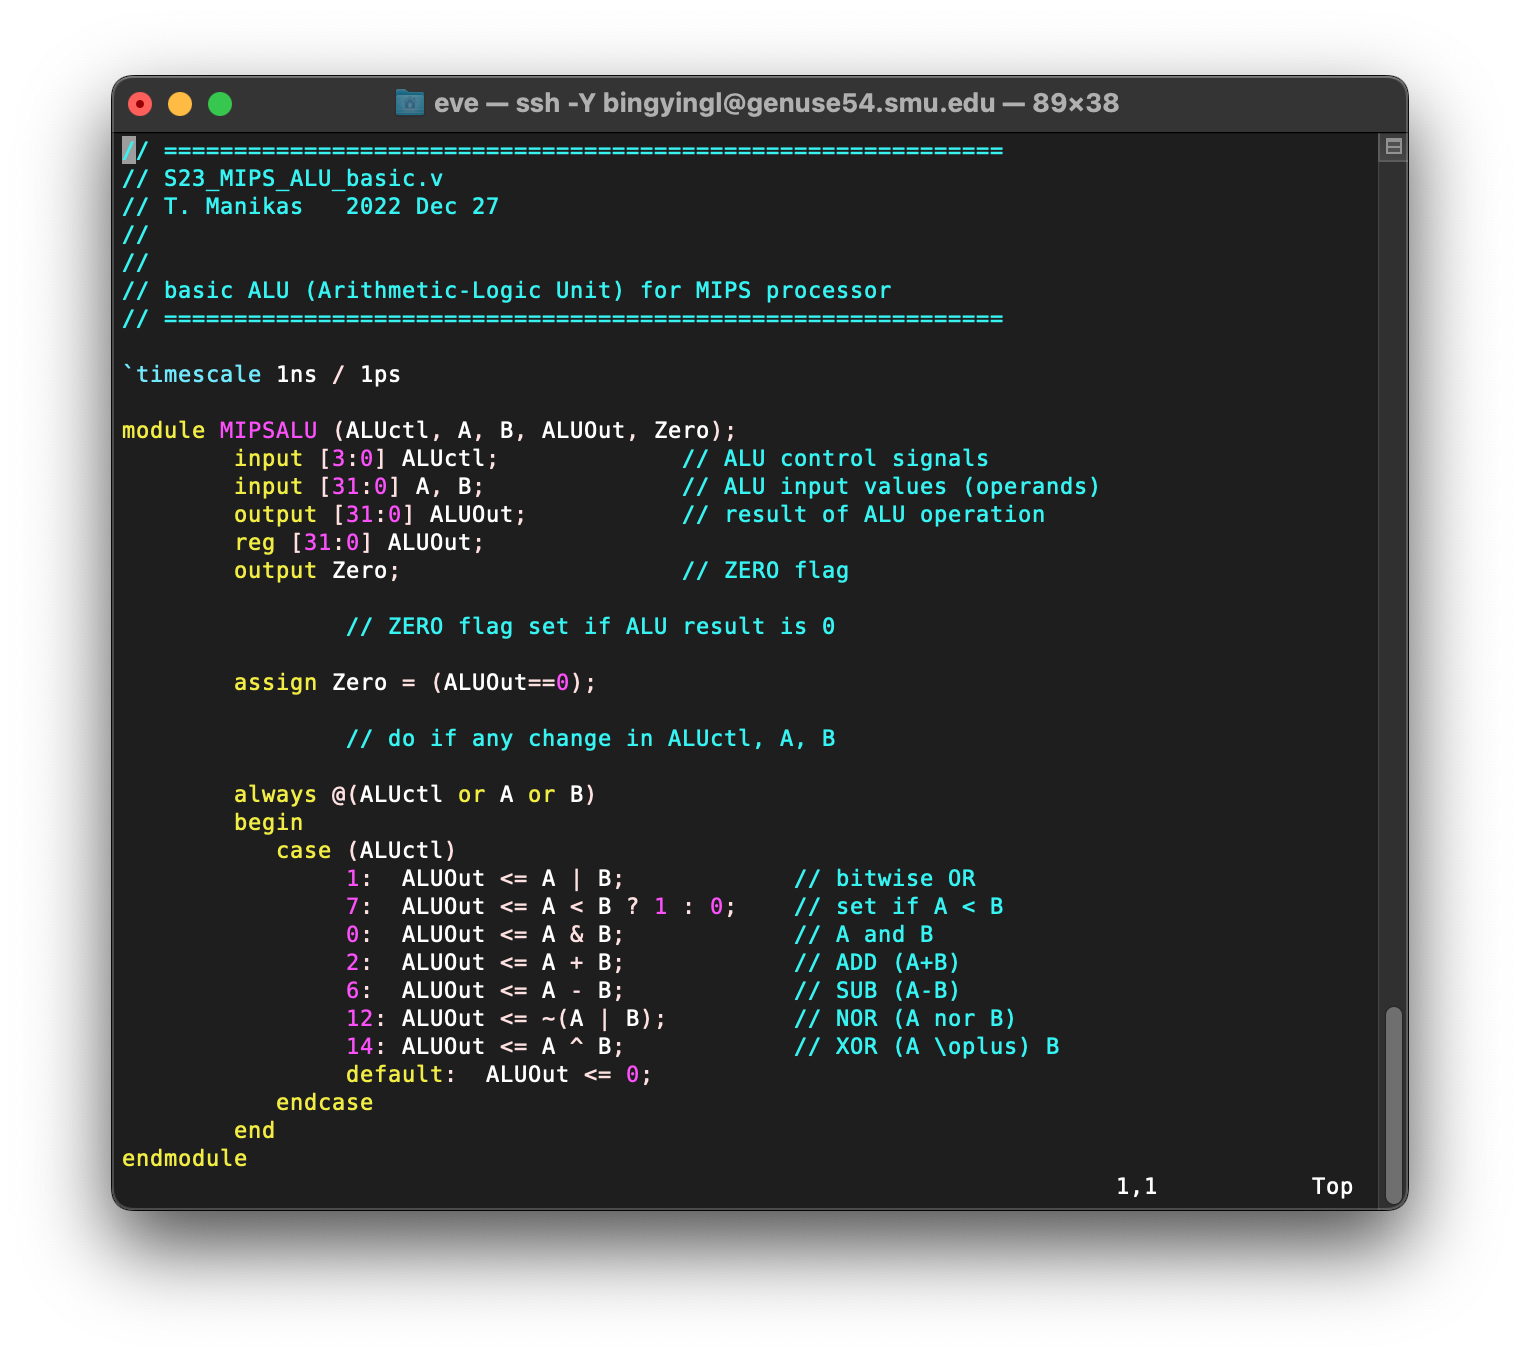
\includegraphics[width=0.9\textwidth]{p2.png}
    \end{center}
    
    \item Please download the following Verilog file:
    \begin{enumerate}
        \item \href{https://smu.instructure.com/courses/106177/files/7254941?wrap=1}{S23\_MIPS\_ALU\_soln\_tb.v} - the testbench for testing your updated ALU
    \end{enumerate}
    \begin{center}
        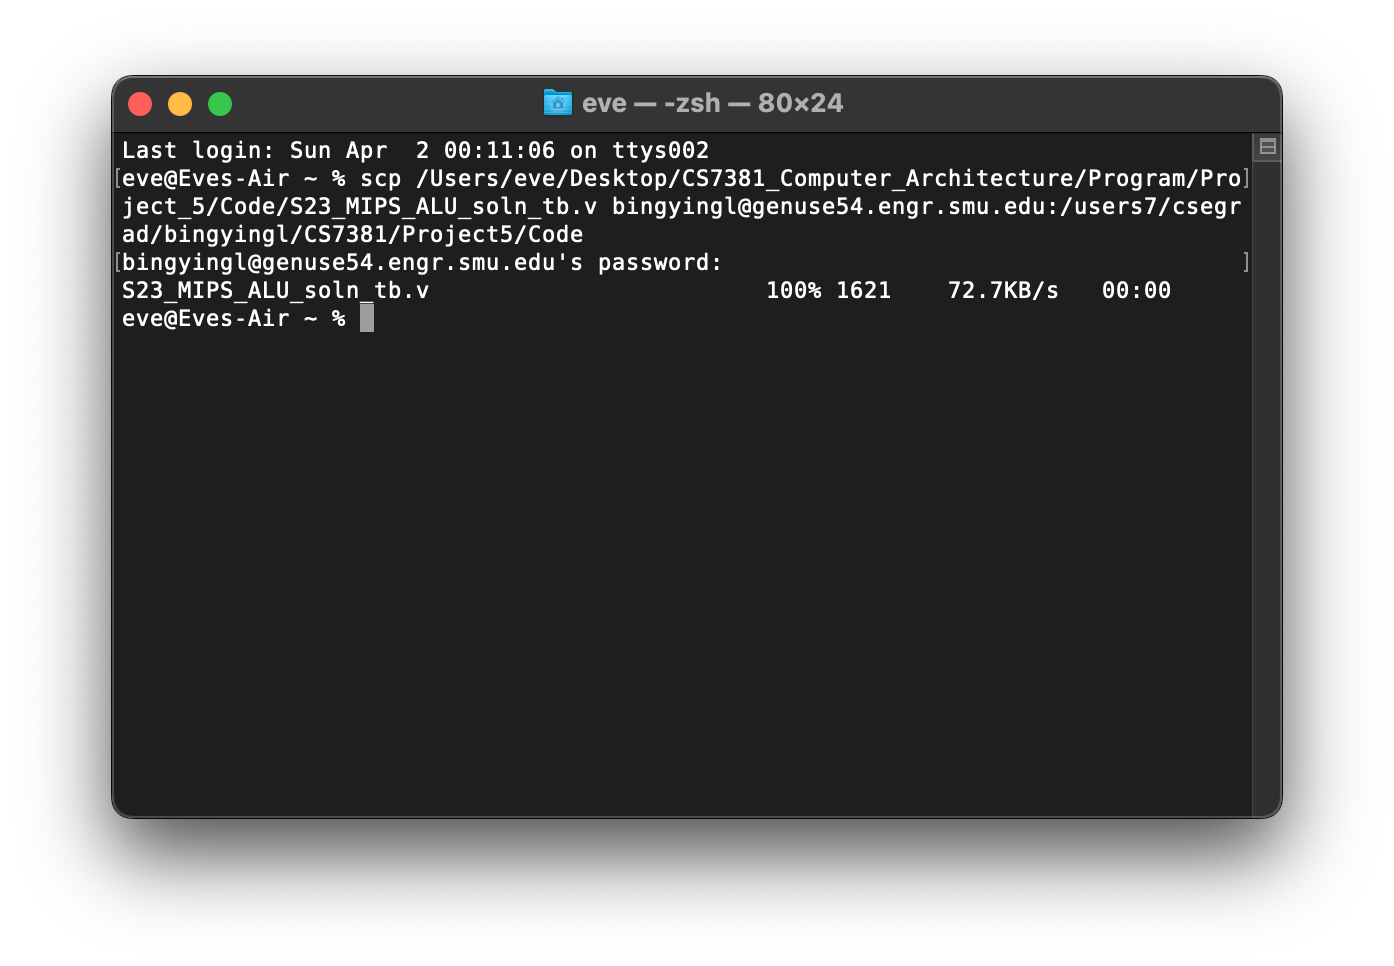
\includegraphics[width=0.9\textwidth]{p3.png}
    \end{center}
    
    \item \textbf{Test your modified ALU using this testbench}
            \begin{center}
        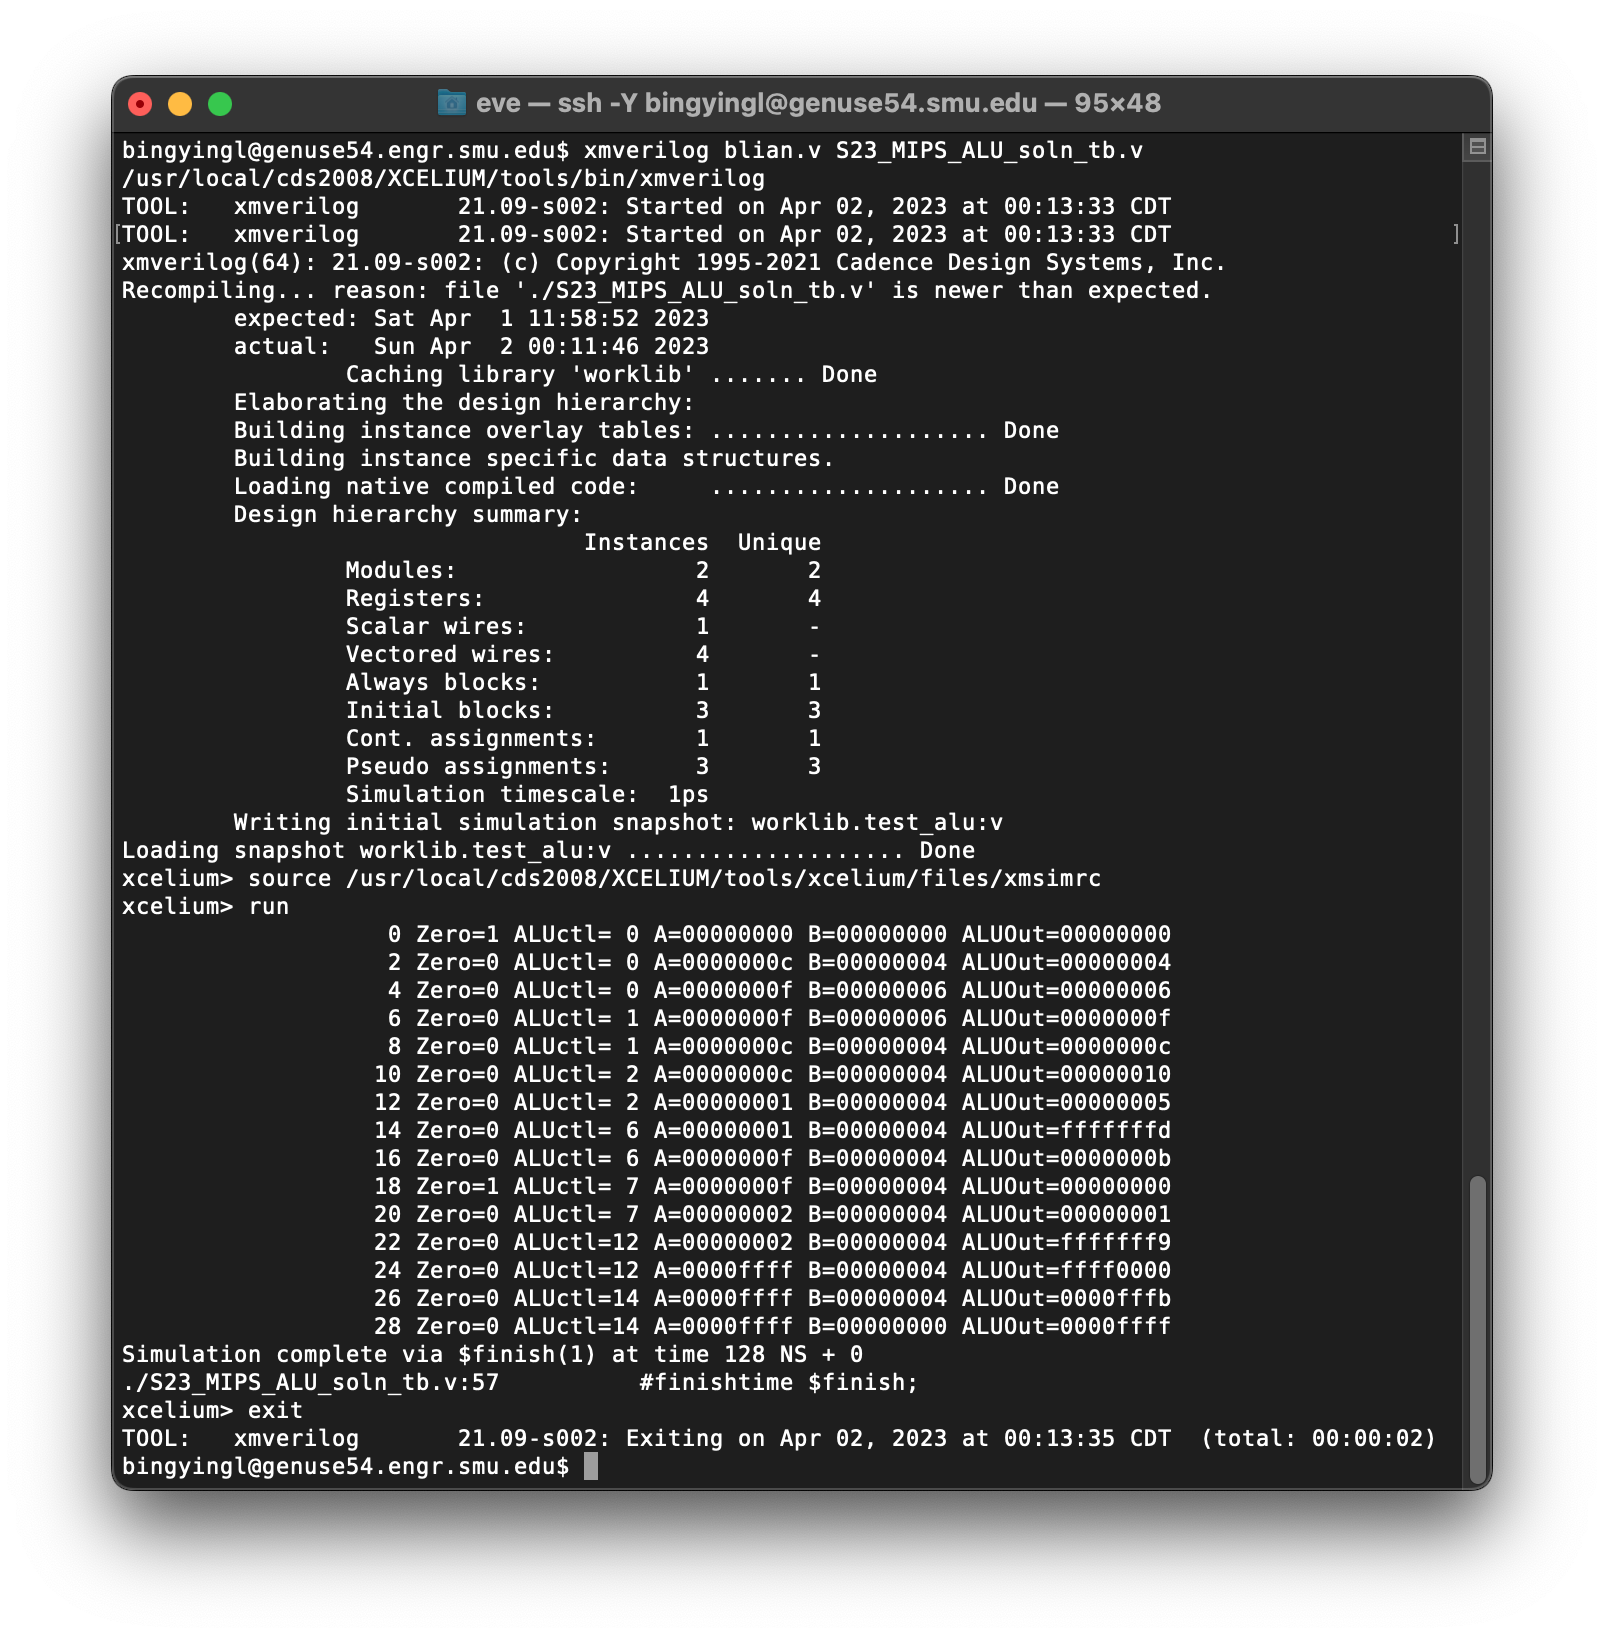
\includegraphics[width=0.9\textwidth]{p4.png}
    \end{center}
    Compare the the result with testbench annotation, they are the same.
                \begin{center}
        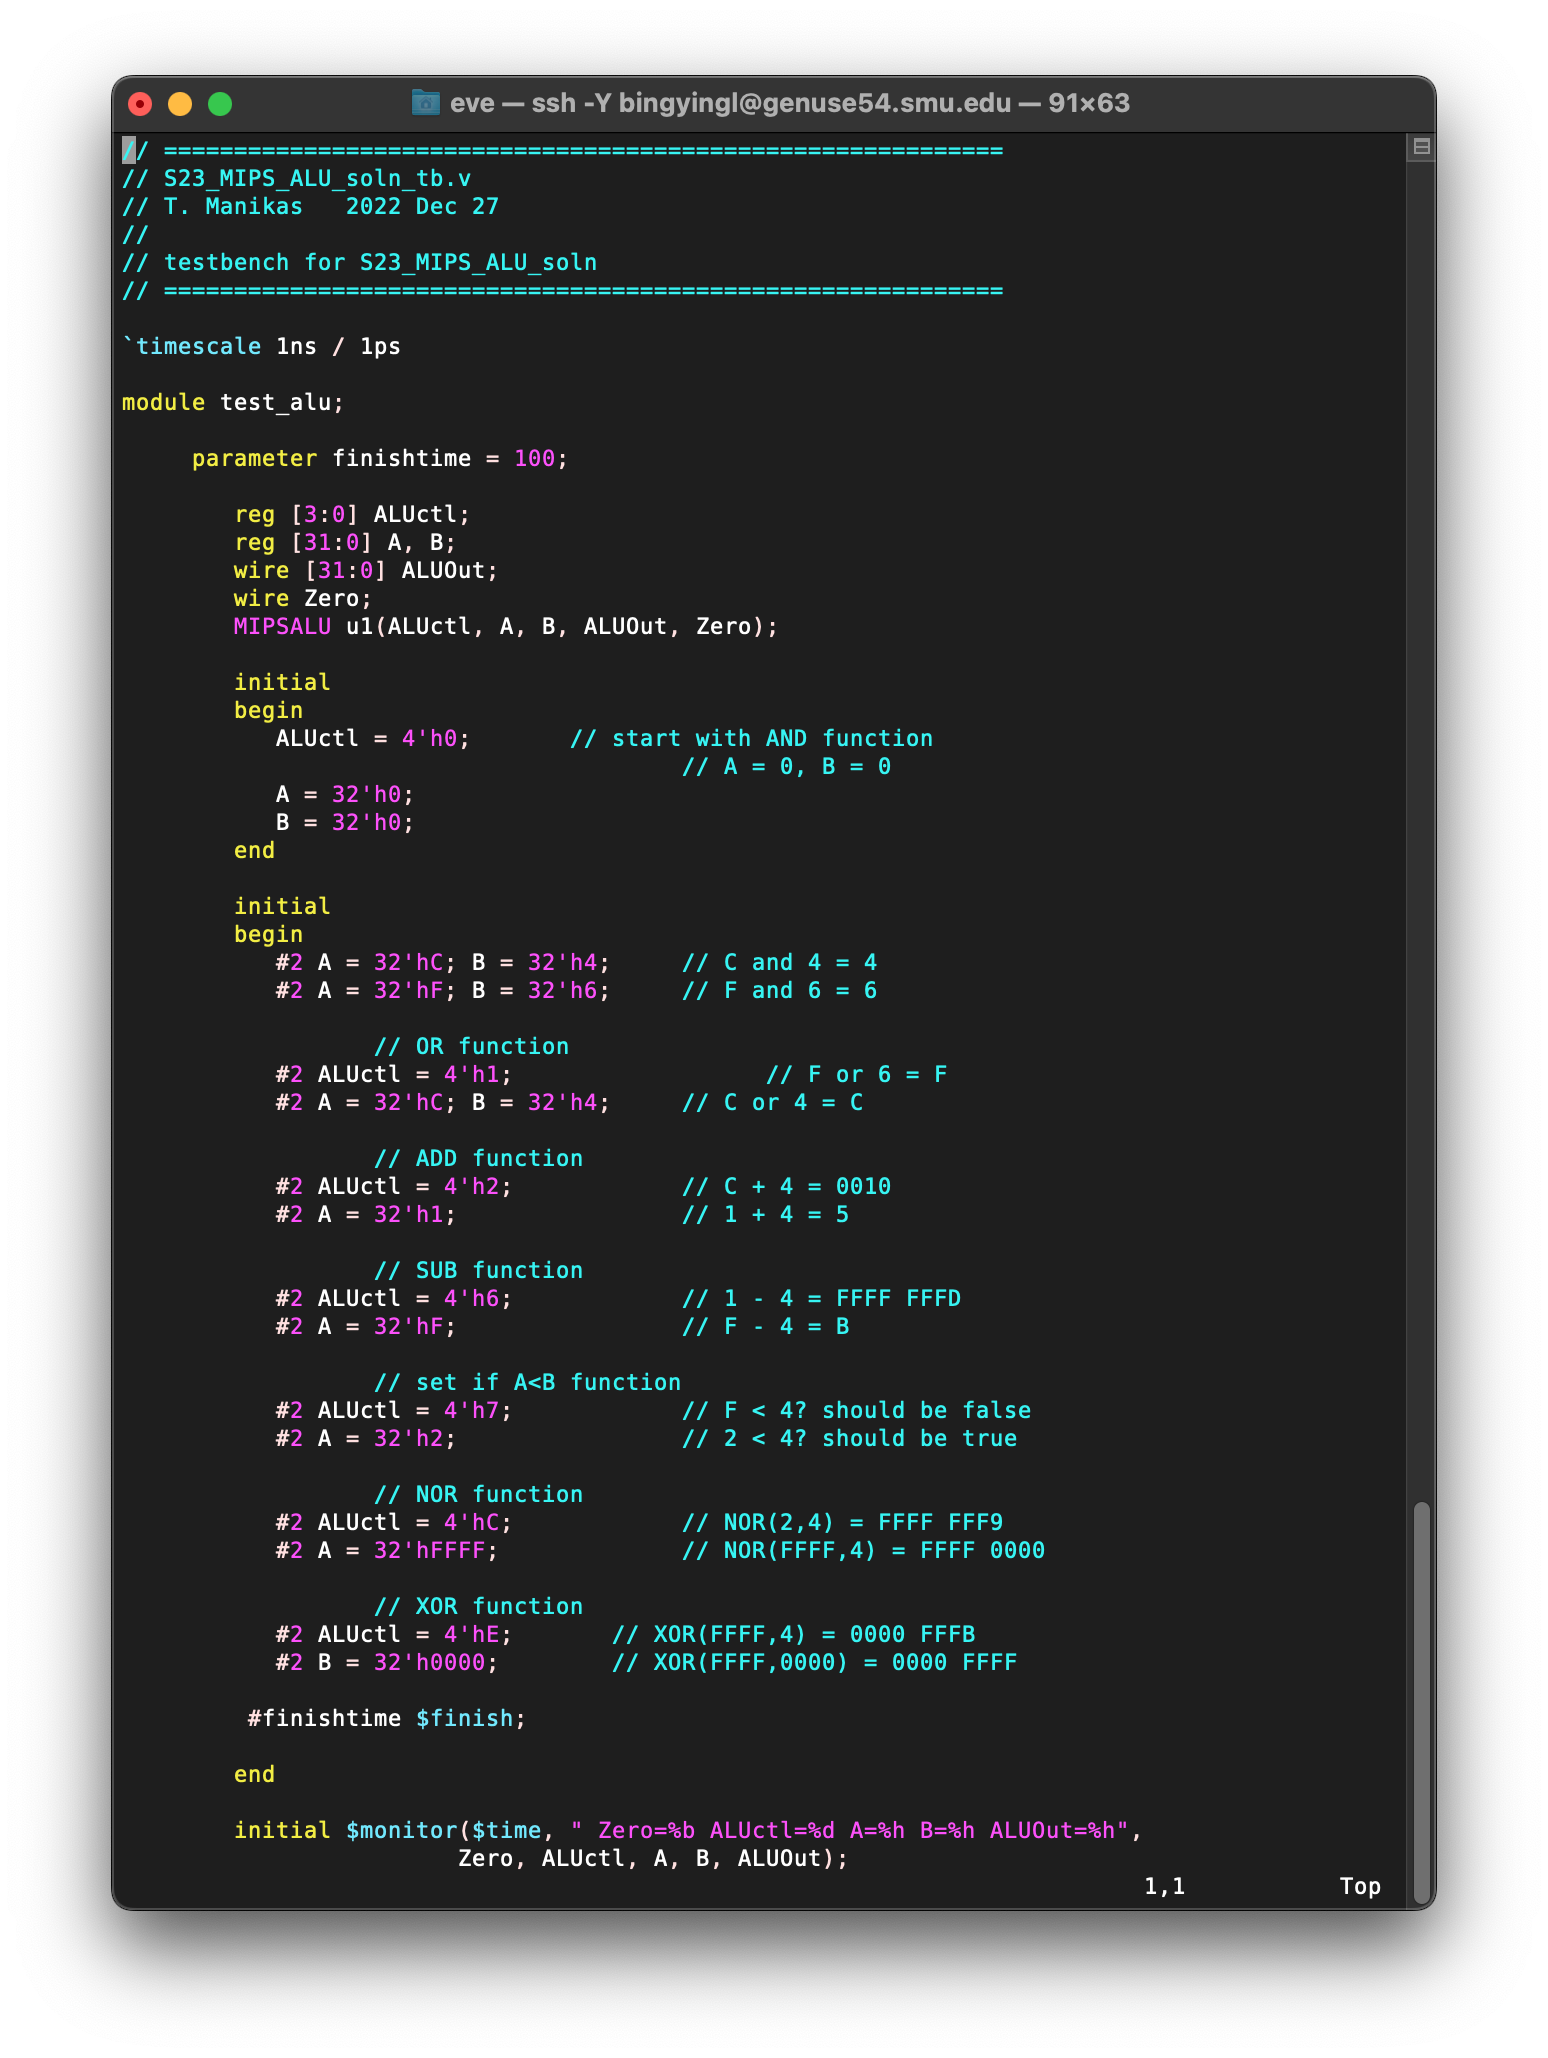
\includegraphics[width=0.9\textwidth]{p5.png}
    \end{center}
    \item \textbf{Please include the following for your homework submission:}
    \begin{enumerate}
        \item Your modified MIPS ALU Verilog file – \textbf{submit the actual *.v file so that the grader can run it.}
                        \begin{center}
        
\includegraphics[width=0.2\textwidth]{p6.png}
    \end{center}
        \item Your testbench results – this can be a copy of the results in a Word document.\\
    \begin{center}
        
\includegraphics[width=0.9\textwidth]{p7.png}
    \end{center}
        I save the result in the document as blian.log
        \item \textbf{PLEASE MAKE SURE THAT YOUR NAME APPEARS ON ALL SUBMITTED ITEMS FOR PROPER CREDIT}
    \end{enumerate}
    
\end{enumerate}

\end{document}
